\documentclass[11pt,a4paper]{article}

\usepackage{lipsum}
\usepackage{multicol}
\usepackage[margin={2cm,2cm}]{geometry}
\setlength{\columnsep}{1cm}
\usepackage{amsmath}
\usepackage{amsfonts}
\usepackage{mathtools}

\newcommand{\R}{\mathbb{R}} % Real set
\newcommand{\Rn}{\mathbb{R}^n}
\newcommand{\Rm}{\mathbb{R}^m}
\newcommand{\Rmn}{\mathbb{R}^{m \times{} n}}
\newcommand{\M}{\mathcal{M}} % Matrix set
\newcommand{\inv}[1]{#1^{-1}} % Inverse
\newcommand{\tr}[1]{#1^{\top}} % Transpose
\newcommand{\inmatrix}[1]{\left(\begin{smallmatrix} #1 \end{smallmatrix} \right)} % Inline small matrix
% requires mathtools
\DeclarePairedDelimiterX{\inner}[2]{\langle}{\rangle}{#1, #2} % Inner product

\begin{document}

\title{Multiple View Geometry}
\author{Course by Daniel Cremers --- written by Matthieu Pizenberg}
\date{June 2017}

\maketitle

\tableofcontents
\clearpage

\begin{multicols}{2}

\section[Linear Algebra]{Mathematical Background: Linear Algebra}
\label{sec:linear_algebra}

This is intended as being a short crash course of linear algebra.

\subsection{Vector Spaces}
\label{sub:vector_spaces}

A set $V$ is called a \textbf{linear space}
or a \textbf{vector space over the field} $\R$
if it is closed under vector summation and scalar multiplication.
\begin{align*}
	+ &: V \times V \rightarrow V \\
	\cdot &: \R \times V \rightarrow V 
\end{align*}

\noindent
With respect to addition ($+$) it forms a commutative group
(existence of neutral element $0$, inverse element $-v$).
Scalar multiplication respects the structure of $\R$ 
($\alpha(\beta v) = (\alpha \beta )v$).
Multiplication and addition respect the \textbf{distributive law}:
\begin{align*}
	( \alpha + \beta )v &= \alpha v + \beta v \\
	\alpha (u + v) & = \alpha u + \alpha v
\end{align*}

\noindent
A subset $W \subset V$ of a vector space $V$
is called a \textbf{subspace} if $0 \in W$ and
$W$ is closed under $+$ and $\cdot$ (for all $\alpha \in \R$).\\

\noindent
A \textbf{spanned subspace} of a set of vectors
$S = \{v_1, \hdots, v_k\} \subset V$ is the subspace
formed by all linear combinations of these vectors.
The set $S$ is called \textbf{linearly independant} if:
\[
	\sum_{i=1}^k \alpha_i v_i = 0 \implies \forall i, \alpha_i = 0
\]
\noindent
A set $B = \{v_1, \hdots, v_n\}$ is called
a \textbf{basis} of $V$ if it is linearly independent and if it
spans the vector space $V$.
A basis is a maximal set of linearly independent vectors.


\subsubsection{Properties of a Basis}
\label{ssub:properties_of_a_basis}

Let $B$ and $B'$ be two bases of a linear space $V$.

\begin{enumerate}
	\item $B$ and $B'$ contain the same number of vectors.
	This number $n$ is called the \textbf{dimension of the space} $V$.

\item Any vector $v \in V$ can be \textbf{uniquely expressed}
	as a linear combination of the basis vectors in
	$B = \{b_1, \hdots, b_n\}$:
	\[
		v = \sum_{i=1}^n \alpha_i b_i
	\]
	\item In particular, all vectors of $B'$ can be expressed as
	linear combinations of vectors of $B$:
	\[
		b'_j = \sum_{i=1}^n \alpha_{ij} b_i
	\]
	The coefficients $\alpha_{ij}$ for this \textbf{basis transform}
	can be combined in a matrix $A$:
	\[
		B' = BA \Leftrightarrow B = B'A^{-1}
	\]
\end{enumerate}


\subsubsection{Inner Product}
\label{ssub:inner_product}

On a vector space, one can define an \textbf{inner product}
(or \textbf{dot product}):
\[\inner{\cdot}{\cdot} : V \times V \rightarrow \R\]
wich is defined by three properties:
\begin{enumerate}
	\item \textbf{linear}:
		$\inner{u}{\alpha v + \beta w} = \alpha \inner{u}{v} + \beta \inner{u}{w}$

	\item \textbf{symmetric}:
		$\inner{u}{v} = \inner{v}{u}$

	\item \textbf{positive definite}:\\
		$\inner{v}{v} \geq 0$ and $\inner{v}{v} = 0 \Leftrightarrow v = 0$
	
\end{enumerate}

\noindent
The scalar product induces a \textbf{norm}:
\[|\cdot| : V \rightarrow \R, \quad |v| = \sqrt{\inner{v}{v}}\]

\noindent
and a \textbf{metric}:
\[d : V \times V \rightarrow \R, \quad d(v,w) = |v - w| = \sqrt{\inner{v-w}{v-w}}\]

\noindent
A vector space with an inner product is then also
a \textbf{metric space}. It is called a \textbf{Hilbert space}.


\subsubsection{Canonical and Induced Inner Product}
\label{ssub:canonical_and_induced_inner_product}

On $V = \R^n$, one can define the canonical inner product for
the canonical basis $B = I_n$ as:

\[\inner{x}{y} = x^{\top} y = \sum_{i=1}^n x_i y_i\]

\noindent
which induces the standard $L_2$-norm or Euclidean norm:

\[|x|_2 = \sqrt{x^{\top}x} = \sqrt{x_1^2 + \hdots + x_n^2}\]

\noindent
With a basis transform $A$ to the new basis $B'$ given by
$B' = IA$ the canonical inner product in the new coordinates
$x'$, $y'$ is given by:

\[\inner{x}{y} = x^{\top} y = {(Ax')}^{\top} (Ay')
= x'^{\top} A^{\top} Ay' \equiv \inner{x'}{y'}_{A^{\top} A}\]

\noindent
The latter product is called the \textbf{induced inner product}
from the matrix $A$.\\

\noindent
Two vectors $v$ and $w$ are \textbf{orthogonal} iff\\
$\inner{v}{w} = 0$.


\subsubsection{Kronecker Product and Stack of a Matrix}
\label{ssub:kronecker_product_and_stack_of_a_matrix}

Given two matrices $A \in \R^{m\times n}$ and $B \in \R^{k \times l}$,
one can define their \textbf{Kronecker product} by:

\[A \otimes B \equiv
	\begin{pmatrix}
		a_{11}B & \cdots & a_{1n}B \\
		\vdots & \ddots & \vdots \\
		a_{m1}B & \cdots & a_{mn}B \\
	\end{pmatrix}
\]
\noindent
In matlab: $C = \mathrm{kron}(A,B)$.

\noindent
Given a matrix $A \in \R^{m \times n}$, its \textbf{stack} $A^s$
is obtained by stacking its $n$ column vectors $a_1, \ldots, a_n \in \R^m$:

\[A^s \equiv
	\begin{pmatrix}
		a_1 \\
		\vdots \\
		a_n \\
	\end{pmatrix}
\in \R^{mn}\]

\noindent
These notations allow to rewrite algebraic expressions, for example:

\[u^{\top} A v = {( v \otimes u )}^{\top} A^s\]

\subsection{Linear Transformations and Matrices}
\label{sub:linear_transformations_and_matrices}

A \textbf{linear transformation} $L$ between tow linear spaces
$V$ and $W$ is a map $L : V \rightarrow W$ such that:
\begin{align*}
	\forall (x,y) \in V^2 ,\quad L(x+y) &= L(x) + L(y) \\
	\forall x \in V, \forall \alpha \in \R,\quad L(\alpha x) &= \alpha L(x)
\end{align*}

\noindent
Due to the linearity, the action of $L$ on the space $V$
is uniquely defined by its action on the basis vectors of $V$.
In the canonical basis ${e_1, \ldots, e_n}$ we have:

\[\forall x \in V, \quad L(x) = Ax\]
\noindent
where
\[A = (L(e_1), \ldots, L(e_n)) \in \R^{m \times n}\]

\noindent
The set of all $m \times n$ matrices is denoted by $\M(m,n)$.
In case that $m = n$, the set $\M(m,n) \equiv \M(n)$
forms a \textbf{ring} over the field $\R$, i.e.\ it is closed
under matrix multiplication and summation.


\subsubsection{The Linear Groups $GL(n)$ and $SL(n)$}
\label{ssub:the_linear_groups_gl_n_and_sl_n_}

A \textbf{group} is a set $G$ with an operation
$\circ : G \times G \rightarrow G$ such that:
\begin{enumerate}
	\item It is closed:
		$\forall (g_1, g_2) \in G^2, \quad g_1 \circ g_2 \in G$
	\item It is associative:
		$\forall (g_1, g_2, g_3) \in G^3, \quad
		(g_1 \circ g2) \circ g_3 = g_1 \circ (g_2 \circ g_3)$
	\item There is a neutral element:
		$\exists e \in G: \forall g \in G, \quad
		e \circ g = g \circ e = g$
	\item Each element has an inverse:
		$\forall g \in G, \exists \inv{g} \in G : \quad
		g \circ \inv{g} = \inv{g} \circ g = e$
\end{enumerate}

\noindent
All invertible (non-singular) real $n \times n$ matrices
form a group with respect to matrix multiplication.
This group is called the \textbf{general linear group} $GL(n)$.
It consists of all $A \in \M(n)$ for which $\det(A) \ne 0$.\\

\noindent
All matrices $A \in GL(n)$ for which $\det(A) = 1$ form a group
called the \textbf{special linear group} $SL(n)$.


\subsubsection{Matrix Representation of Groups}
\label{ssub:matrix_representation_of_groups}

A group $G$ has a \textbf{matrix representation} or can be realized as
a matrix group if there exists an injective transformation:

\[R : G \rightarrow GL(n)\]

\noindent
which \textbf{preserves the group structure} of $G$,
that is inverse and composition are preserved by the map:

\begin{align*}
	R(e) &= I_{n \times n} \\
	\forall (g,h) \in G^2, \quad R(g\circ h) &= R(g)R(h)
\end{align*}

\noindent
Such a map $R$ is called a \textbf{group homomorphism}.
The idea is to study properties of the group by the matrices properties.


\subsubsection{The Affine Group $A(n)$}
\label{ssub:the_affine_group_a_n_}

An affine transformation $L : \R^n \rightarrow \R^n$
is defined by a matrix $A \in GL(n)$ and a vector $b \in \R^n$ such that:
\[L(x) = Ax + b\]

\noindent
The set of all such affine transformations is called the
\textbf{affine group of dimension $n$}, denoted by $A(n)$.
L defined above is not a linear map unless $b=0$.
By introducing \textbf{homogeneous coordinates} to represent $x \in \R^n$ by
$\inmatrix{x \\ 1} \in \R^{n+1}$,
$L$ becomes a linear mapping from:

\[L: \R^{n+1} \rightarrow \R^{n+1}; \quad
	\begin{pmatrix}
		x \\
		1 \\
	\end{pmatrix}
	\mapsto
	\begin{pmatrix}
		A & b \\
		0 & 1 \\
	\end{pmatrix}
	\begin{pmatrix}
		x \\
		1 \\
	\end{pmatrix}\]

\noindent
A matrix $\inmatrix{A & b \\ 0 & 1}$ with $A \in GL(n)$ and $b \in R^n$
is called an \textbf{affine matrix}. It is an element of $GL(n+1)$.
The affine matrices form a subgroup of $GL(n+1)$.


\subsubsection{The Orthogonal Group $O(n)$}
\label{ssub:the_orthogonal_group_o_n_}

A matrix $A \in \M(n)$ is called \textbf{orthogonal} if it preserves
the inner product:
\[\forall (x,y) \in {(\R^n)}^2 \quad \inner{Ax}{Ay} = \inner{x}{y}\]

\noindent
The set of all orthogonal matrices forms the \textbf{orthogonal group}
$O(n)$, which is a subgroup of $GL(n)$.
For an orthogonal matrix $R$ we have:
\[\forall (x,y) \in {(\R^n)}^2, \quad
\inner{Rx}{Ry} = \tr{x}\tr{R}Ry = \tr{x}y\]

\noindent
Therefore, we must have $\tr{R}R = R\tr{R} = I$, i.e.
\[O(n) = \{ R \in GL(n) \ | \ \tr{R}R = I \}\]

\noindent
We can show that $\det(R) \in \{ \pm 1\}$.
The subgroup of $O(n)$ with $\det(R) = +1$ is called
the \textbf{special orthogonal group} $SO(n)$.
$SO(n) = O(n) \cap SL(n)$.
In particular, $SO(3)$ is the group of all 3-dimensional rotation matrices.


\subsubsection{The Euclidean Group $E(n)$}
\label{ssub:the_euclidean_group_e_n_}

A Euclidean transformation $L$ from $\R^n$ to $\R^n$ is defined by
an orthogonal matrix $R \in O(n)$ and a vector $T \in R^n$:
\[L : \R^n \rightarrow \R^n; \quad x \mapsto Rx + T\]

\noindent
The set of all such transformations is called the
\textbf{Euclidean group} $E(n)$. It is a subgroup of the affine group $A(n)$.
\[E(n) = \left\{
	\begin{pmatrix}
		R & T \\
		0 & 1 \\
	\end{pmatrix}
\ \middle| \ R \in O(n), \ T \in \R^n \right\}\]


\noindent
If $R \in SO(n)$ then we have the \textbf{special euclidean group} $SE(n)$.
In particular, $SE(3)$ represent the \textbf{rigid-body motions} in $\R^3$.\\

\noindent
In summary:

\[\boxed{SO(n) \subset O(n) \subset GL(n)}\]
\[\boxed{SE(n) \subset E(n) \subset A(n) \subset GL(n+1)}\]


\subsection{Properties of Matrices}
\label{sub:properties_of_matrices}


\subsubsection{Range, Span, Null Space and Kernel}
\label{ssub:range_span_null_space_and_kernel}

Let $A \in \Rmn$ be a matrix defining a linear map from $\Rn$ to $\Rm$.
The \textbf{range} or \textbf{span} of $A$ is defined as the subspace
of $\Rm$ which can be ``reached'' by $A$:
\[\text{range}(A) = \{ y \in \Rm \ |\  \exists x \in \Rn : Ax = y \}\]

\noindent
The range of a matrix $A$ is given by the span of its column vectors.
The \textbf{null space} or \textbf{kernel} of a matrix $A$ is given by
the subset of vectors $x \in \Rn$ which are mapped to zero:
\[\text{null}(A) \equiv \ker(A) = \{ x \in \Rn \ | \ Ax = 0 \}\]

\noindent
The null space of a matrix $A$ is given by the vectors
orthogonal to its row vectors. In matlab: $Z = \text{null}(A)$.
The concepts of range and null space are useful when studying the
\textbf{solution of linear equations}. The system $Ax = b$ will have
a solution $x \in \Rn$ if and only if $b \in \text{range}(A)$.
Moreover, this solution will be unique only if $\ker(A) = \{0\}$.\\

\noindent
The \textbf{rank} of a matrix is the dimension of its range:
\[\text{rank}(A) = \dim(\text{range}(A))\]

\noindent
The rank of a matrix $A \in \Rmn$ has the following properties:
\begin{enumerate}
	\item $\text{rank}(A) = n - \dim(\ker(A))$
	\item $0 \le \text{rank}(A) \le \min\{m,n\}$.
	\item $\text{rank}(A)$ is equal to the maximum number
		of linearly independent row (or column) vectors of $A$.
	\item $\text{rank}(A)$ is the highest order of a nonzero minor of $A$,
		where a \textbf{minor of order k} is the determinant
		of a $k \times k$ submatrix of $A$.
	\item \textbf{Sylvester's inequality}: Let $B \in \R^{n \times k}$.
		then $AB \in \R^{m \times k}$ and
		$\text{rank}(A) + \text{rank}(B) - n \le
			\text{rank}(AB) \le \min \{ \text{rank}(A), \text{rank}(B)\}$.
	\item For any nonsingular matrices $C \in \R^{m \times m}$
		and $D \in \R^{n \times n}$, we have:
		$\text{rank}(A) = \text{rank}(CAD)$.
\end{enumerate}

\clearpage

\section{Representing a Moving Scene}%
\label{sec:moving_scene}


\subsection{The Origins of 3D Reconstruction}%
\label{sub:the_origins_of_3d_reconstruction}

The goal to reconstruct the three-dimensional structure of the world from
a set of two-dimensional views has long history in computer vision.
It is a classical \textbf{ill-posed problem}, because the reconstruction
consistent with a given set of observations/images is typically not unique.
Therefore, one will need to impose additional assumptions.
Mathematically, the study of geometric relations between a 3D scene
and the observed 2D projections is based on two types of transformations, namely:
\begin{itemize}
	\item \textbf{Euclidean motion} or \textbf{rigid body motion}
		representing the motion of the camera from one frame to the next.
	\item \textbf{Perspective projection} to account for the image formation
		process (see pinhole camera, etc).
\end{itemize}

The notion of perspective projection has its roots among the ancient Greeks
(Euclid of Alexandria, \roughly{} 400 B.C.) and the Renaissance period
(Brunelleschi \& Alberti, 1435).
The study of perspective projection lead to the field of
\textbf{projective geometry} (Girard Desargues 1648, Gaspard Monge 18th cent).\\

The first work on the problem of multiple view geometry was that of
\textbf{Erwin Kruppa (1913)} who showed that two views of five points
are sufficient to determine both the relative tansformation
(\textbf{motion}) between the two views and the 3D location (\textbf{structure})
of the points up to finitely many solutions.\\

A linear algorithm to recover structure and motion from two views based
on the epipolar constraint was proposed by \textbf{Longuet-Higgins}
in \textbf{1981}. An entire series of works along these lines was summarized
in several text books (Faugeras 1993, Kanatani 1993,
Maybank 1993, Weng et al. 1993).\\

Extensions to three views were developed by Spetsakis and Aloimonos '87, '90
, and by Shashua '94 and Hartley '95.
Factorization techniques for multiple views and orthogonal projection were
developed by Tomasi and Kanade 1992.\\

The joint estimation of camera motion and 3D location is called
\textbf{structure and motion} or \textbf{visual SLAM}.


\subsection{3D Space \& Rigid Body Motion}%
\label{sub:3d_space_rigid_body_motion}


\subsubsection{Three-dimensional Euclidean Space}%
\label{ssub:three_dimensional_euclidean_space}

The three-dimensional Euclidean space $\E^3$ consists of all points
$p \in \E^3$ characterized by coordinates
	\[\bm{X} \equiv \tr{(X_1, X_2, X_3)} \in \R^3\]

such that $\E^3$ can be identified with $\R^3$.
That means we talk about points ($\E^3$) and coordinates ($\R^3$)
as if they were the same thing. Given two points $\bm{X}$ and $\bm{Y}$,
one can define a \textbf{bound vector} as
	\[v = \bm{Y} - \bm{X} \in \R^3\]

Considering this vector independent of its base point $\bm{Y}$ makes
it a \textbf{free vector}. The set of free vectors $v \in \R^3$
forms a linear vector space. By identifying $\E^3$ and $\R^3$,
one can endow $\E^3$ with a scalar product, a norm and a metric.
This allows to compute \textbf{distances, curve length, areas or volumes.}
\[\text{For a curve } \gamma : [0,1] \rightarrow \R^3,\quad
	l(\gamma) \equiv \int_{0}^1 | \dot{\gamma}(s) | d\!s\]


\subsubsection{Cross Product \& Skew-symmetric Matrices}%
\label{ssub:cross_product_and_skew_symmetric_matrices}

On $\R^3$ one can define a cross product
\[\times : \R^3 \times \R^3 \rightarrow \R^3,\quad u \times v =
	\begin{pmatrix}
		u_2v_3 - u_3v_2 \\
		u_3v_1 - u_1v_3 \\
		u_1v_2 - u_2v_1
	\end{pmatrix} \in \R^3\]

which is a vector \textbf{orthogonal to $u$ and $v$}.
Since $u \times v = -v \times u$, the cross product introduces an \textbf{orientation}.
Fixing $u$ induces a linear mapping $v \mapsto u \times v$ wich
can be represented by the \textbf{skew-symmetric matrix}
\[\widehat{u} = \hatmat{u_1}{u_2}{u_3} \in \RR{3}{3}\]

In turn, every skew symmetric matrix $M = -\tr{M} \in \RR{3}{3}$
can be identified with a vector $u \in \R^3$.
The operator $\widehat{}$ defines an \textbf{isomorphism} between $\R³$
and the space $so(3)$ of the $3 \times 3$ skew-symmetric matrices.
Its inverse is denoted by $\vee : so(3) \rightarrow \R^3$.


\subsubsection{Rigid-body Motion}%
\label{ssub:rigid_body_motion}

A \textbf{rigid-body motion} (or rigid-body transformation)
is a family of maps
\[g_t : \R^3 \rightarrow \R^3;\quad \bm{X} \mapsto g_t(\bm{X}),\quad t \in [0,T]\]

which preserve the norm and cross product of any two vectors:
\begin{itemize}
	\setlength\itemsep{-0.2em}
	\item $\forall v \in \R^3, \quad |g_t(v)| = |v|$
	\item $\forall u,v \in \R^3, \quad g_t(u) \times g_t(v) = g_t(u \times v)$
\end{itemize}

Since norm and scalar product are related by the \textbf{polarization identity}
\[\inner{u}{v} = \frac{1}{4}(|u+v|^2 - |u-v|^2)\]

one can also state that a rigid-body motion is a map which
preserves inner product and cross product.
As a consequence, rigid-body motions also preserves the \textbf{triple product}
\[\forall u, v, w \in \R^3, \quad
	\inner{g_t(u)}{g_t(v) \times g_t(w)} = \inner{u}{v \times w}\]

which means that they are volume-preserving.


\subsubsection{Representation of Rigid-body Motion}%
\label{ssub:representation_of_rigid_body_motion}

Let $g_t$ our rigid body motion. We are going to detail what this transformation
is doing to the initial frame of orthonormal oriented vecors
$e_1, e_2, e_3 \in \R^3$.
We note the transformed vectors $r_i = g_t(e_i)$.
Scalar and cross product of these vectors are preserved:
	\[\tr{r_i}r_j = \tr{g_t(e_i)}g_t(e_j) = \tr{e_i}e_j = \delta_{ij}, \quad
	r_1 \times r_2 = r_3\]

The first constraint amounts to the statement that the matrix
$R = (r_1, r_2, r_3)$ is an orthogonal matrix: $\bm{\tr{R}R=R\tr{R}=I}$,
whereas the second property implies that $\bm{\det(R) = +1}$.
In other words: $R$ is an element of the group
$SO(3) = \{R \in \RR{3}{3}\ |\ \tr{R}R=I,\ \det(R) = +1\}$.\\

The motion of the origin can be represented by a \textbf{translation}
$\bm{T \in R^3}$. Thus the rigid body motion $g_t$ can be written as:
	\[g_t(x) = Rx + T\]


\subsubsection{Exponential Coordinates of Rotation}%
\label{ssub:exponential_coordinates_of_rotation}

We will now derive a representation of an \textbf{infinitesimal rotation}.
To this end, we consider a family of rotation matrices $R(t)$
which continuously transform a point from its original location
$(R(0) = I)$ to a different one.
	\[\bm{X}_{\text{trans}}(t) = R(t)\bm{X}_{\text{orig}}, \quad
	\text{with } R(t) \in SO(3)\]

Since $\forall t,\ R(t)\tr{R(t)} = I$, we have:
	\[\frac{d}{dt}(R\tr{R}) = \dot{R}\tr{R} + R\tr{\dot{R}}= 0
	\implies \dot{R}\tr{R} = -\tr{( \dot{R}\tr{R} )}\]

Thus, $\dot{R}\tr{R}$ is a \textbf{skew-symmetric matrix}.
As shown in the section about the $\widehat{}$ operator, this implies that
there exists a vector $w(t) \in \R^3$ such that:
	\[\dot{R}(t)\tr{R}(t) = \widehat{w}(t)
	\Leftrightarrow \bm{ \dot{R}(t) = \widehat{w}(t)R(t)}\]

Since $R(0) = I$, it follows that $\dot{R}(0) = \widehat{w}(0)$.
Therefore, the \textbf{skew-symmetric matrix $\bm{\widehat{w}(0) \in so(3)}$
gives the first order approximation of a rotation:}
	\[R(dt) = R(0) + dR = I + \widehat{w}(0) dt\]


\subsection{The Lie Group $SO(3)$}%
\label{sub:the_lie_group_so_3_}


\subsubsection{Lie Group and Lie Algebra}%
\label{ssub:lie_group_and_lie_algebra}

The above calculations showed that the effect of any infinitesimal
rotation $R \in SO(3)$ can be approximated by an element from
the space of skew-symmetric matrices
	\[so(3) = \{ \widehat{w}\ |\ w \in \R^3\}\]

The rotation group $SO(3)$ is called a \textbf{Lie group}.
The space $so(3)$ is called its \textbf{Lie algebra}.\\

\underline{Definition:}
A \textbf{Lie group} (or infinitesimal group) is a smooth manifold that
is also a group, such that the group operations multiplication
and inversion are smooth maps.\\

As shown above: \textbf{The Lie algebra $\bm{so(3)}$ is the tangent space
at the identity of the rotation group $\bm{SO(3)}$.}\\

An \textbf{algebra over a field $\bm{K}$} is a vector space $V$ over $K$
with multiplication on the space $V$.
Elements $\widehat{w}$ and $\widehat{v}$ of the Lie algebra
generally do not commute.
One can define the \textbf{Lie bracket}
\[[\cdot,\cdot]: so(3) \times so(3) \rightarrow so(3);\quad
[\widehat{w},\widehat{v}] \equiv \widehat{w}\widehat{v} - \widehat{v}\widehat{w}\]


\subsubsection{Sophus Lie (1841--1899)}%
\label{ssub:sophus_lie_1841_1899_}

\begin{figure}[ht]
\centering
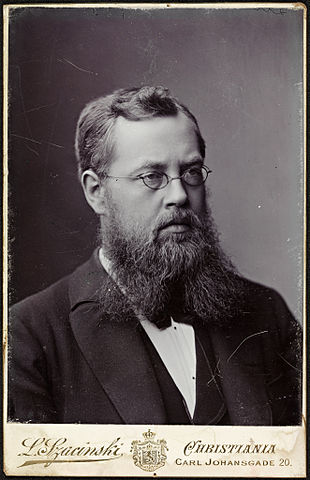
\includegraphics[width=10em]{img/sophus_lie.jpg}
\caption*{Portrait of Marius Sophus Lie}
\end{figure}

Marius Sophus Lie was a Norwegian-born mathematician.
He created the theory of \textbf{continuous symmetry}, and applied it to
the study of geometry and differential equations. Among his greatest
achievements was the discovery that continuous transformation
groups are better understood in their linearized versions
(``Theory of transformation groups'' 1893).
These \textbf{infinitesimal generators} form a structure which is today
known as a \textbf{Lie algebra}. The linearized version of the group law
corresponds to an operation on the Lie algebra known as
the \textbf{commutator bracket} or \textbf{Lie bracket}.
1882 Professor in Christiania (Oslo),
1886 Leipzig (succeeding Felix Klein),
1898 Christiania.


\subsubsection{The Exponential Map}%
\label{ssub:the_exponential_map}

Given the infinitesimal formulation of rotation,
we got to the differential equation system:
	\[\left\{ \begin{aligned}
		\dot{R}(t) &= \widehat{w}(t)R(t) \\
		R(0) &= I \\
	\end{aligned}\right.\]

If we assume that $\widehat{w}(t)$ is constant in time ($=\widehat{w}$),
this known equation has the solution:
	\[R(t) = e^{\widehat{w}t}
		= \sum_{n=0}^{\infty} \frac{{(\widehat{w}t)}^n }{n!}
		= I + \widehat{w}t + \frac{{(\widehat{w}t)}^2 }{2!} + \ldots \]

which is a rotation around the axis $w \in \R^3$
by an angle of t (if $\|w\| = 1$). Alternatively, one can absorb
the scalar $t \in \R$ into the skew  symmetric matrix $\widehat{w}$
to obtain $R(t) = e^{\widehat{v}}$ with $\widehat{v} = \widehat{w}t$.
This \textbf{matrix exponential} therefore defines a map from
the Lie algebra to the Lie group:
	\[\exp : so(3) \rightarrow SO(3);\quad \widehat{w}\mapsto e^{\widehat{w}}\]


\subsubsection{The Logarithm of $SO(3)$}%
\label{ssub:the_logarithm_of_so_3_}

There is conversely a mapping from the Lie group to the Lie algebra.
For any rotation matrix $R \in SO(3)$, there exists a $w \in \R^3$
such that $R = \exp(\widehat{w})$. Such an element is denoted by
$\widehat{w} = \log(R)$. If $R \ne I$, we note $r_{ij}$ its coefficients
and $w$ is given by:
	\[\left\{ \begin{aligned}
		|w| &= \inv{\cos}\left(\frac{\text{trace}(R)-1}{2}\right)\\
		\frac{w}{|w|} &= \frac{1}{2\sin(|w|)}
			\begin{pmatrix}
				r_{32} - r_{23} \\
				r_{13} - r_{31} \\
				r_{21} - r_{12} \\
			\end{pmatrix}
	\end{aligned}\right.\]

For $R = I$, we have $|w| = 0$, i.e.\ a rotation by an angle 0.
The above statement says:
\textbf{Any orthogonal transformation $\bm{\R \in SO(3)}$ can be realized
by rotating by an angle $\bm{|w|}$ around an axis
$\bm{\frac{w}{|w|}}$ as defined above}.\\

Obviously the above representation is not unique since for example,
increasing the angle by multiples of $2\pi$ will give the same rotation.


\subsubsection{Rodrigues' Formula}%
\label{ssub:rodrigues_formula}

In analogy to the well-known Euler equation
	\[\forall \phi \in \R, \quad  e^{i\phi} = \cos(\phi) + i\ \sin(\phi)\]

we have an expression for skew symmetric matrices $\widehat{w} \in so(3)$:
	\[\boxed{
	e^{\widehat{w}} = I + \frac{\widehat{w}}{|w|} \sin(|w|)
		+ \frac{\widehat{w}^2}{|w|^2} (1 - \cos(|w|))}\]

This is known as \textbf{Rodrigues' formula}.\\

\underline{Proof sketch:}
Let $t = |w|$ and $v = w/|w|$ such that $w = vt$. Then one can show that:
	\[\widehat{v}^2 = v\tr{v} - I \quad
	\text{and}\quad \widehat{v}^3 = -\widehat{v}\]
Thus, by developing the exponential, we get:
	\[e^{\widehat{v}t} = I +
		\underbrace{\left( t - \frac{t^3}{3!} + \cdots \right)}_{\sin(t)}\widehat{v}
	+ \underbrace{\left(\frac{t^2}{2!}-\frac{t^4}{4!}+\cdots \right)}_{1-\cos(t)}
		\widehat{v}^2\]


\subsection{The Lie Group $SE(3)$}%
\label{sub:the_lie_group_se_3_}


\subsubsection{Representation of Rigid-body Motions $SE(3)$}%
\label{ssub:representation_of_rigid_body_motions_se_3_}

We have seen that the space of rigid-body motions is given by
the group of special Euclidean transformations:
	\[SE(3) \equiv \{ g = (R,T)\ |\ R \in SO(3),\ T \in \R^3\}\]
In homogeneous coordinates:
	\[\boxed{SE(3) \equiv
	\left\{ g = \begin{pmatrix}
		R & T \\
		0 & 1 \\
	\end{pmatrix}\ \middle|\ R \in SO(3), T \in \R^3\right\}}\]

In the context of rigid motions, one can see the difference
between points in $\E^3$ (which can be rotated and translated)
and vectors in $\R^3$ (which can only be rotated).


\subsubsection{The Lie Algebra of Twists}%
\label{ssub:the_lie_algebra_of_twists}

Given a continuous family of rigid-body transformations:
	\[g : \R \rightarrow SE(3);\quad g(t) = \begin{pmatrix}
		R(t) & T(t) \\
		0 & 1 \\
	\end{pmatrix}\ \in \RR{4}{4}\]

we consider:
	\[\dot{g}(t)\inv{g}(t) = \begin{pmatrix}
		\dot{R}\tr{R} & \dot{T} - \dot{R}\tr{R}T \\
		0 & 0 \\
	\end{pmatrix}\ \in \RR{4}{4}\]

As in the case of $SO(3)$ the $\dot{R}\tr{R}$ corresponds
to some skew-symmetric matrix $\widehat{w} \in so(3)$. Defining a vector
$v(t) = \dot{T}(t) - \widehat{w}(t)T(t)$, we have:
	\[\dot{g}(t)\inv{g}(t) = \begin{pmatrix}
		\widehat{w}(t) & v(t) \\
		0 & 0 \\
	\end{pmatrix} \equiv \widehat{\xi}(t) \in \RR{4}{4}\]

Multiplying with $g(t)$ from the right, we obtain:
	\[\dot{g} = \dot{g}\inv{g}g = \widehat{\xi}g\]

The $4 \times 4$ matrix $\widehat{\xi}$ can be viewed as a tangent vector
along the curve $g(t)$. $\widehat{\xi}$ is called a \textbf{twist}.
As in the case of $so(3)$, the set of all twists forms the tangent
space which is the \textbf{Lie algebra}
	\[\boxed{se(3) \equiv \left\{ \widehat{\xi} = \begin{pmatrix}
		\widehat{w} & v \\
		0 & 0 \\
	\end{pmatrix}\ \middle|
	\ \widehat{w} \in so(3),\ v \in \R^3 \right\}}\]

	to the \textbf{Lie group $\bm{SE(3)}$}.\\

As before, we can define operators $\wedge$ and $\vee$ to convert between
a \textbf{twist $\bm{\widehat{\xi} \in se(3)}$} and its
\textbf{twist coordinates} $\bm{ \xi \in \R^6 }$:
	\[\widehat{\xi} \equiv \begin{pmatrix} v \\ w \end{pmatrix}^{\wedge}
		\equiv \begin{pmatrix}
			\widehat{w} & v \\
			0 & 0
		\end{pmatrix}\ \in \RR{4}{4}\]

	\[\begin{pmatrix}
		\widehat{w} & v \\
		0 & 0
	\end{pmatrix}^{\vee} \equiv \begin{pmatrix} v \\ w \end{pmatrix} \in \R^6\]


\subsubsection{Exponential Coordinates for $SE(3)$}%
\label{ssub:exponential_coordinates_for_se_3_}

The twist coordinates $\xi = \inmatrix{v\\w}$ are formed by stacking the
\textbf{linear velocity} $\bm{v \in \R^3}$ (related to translation) and the
\textbf{angular velocity} $\bm{w \in \R^3}$ (related to rotation).\\

The differential equation system:
	\[\left\{ \begin{aligned}
		\dot{g}(t) &= \widehat{\xi}g(t), \quad \widehat{\xi} = \text{const}\\
		g(0) &= I
	\end{aligned} \right.\]

has the solution $g(t) = e^{\widehat{\xi}t} = \sum_{n=0}^{\infty}
\frac{{(\widehat{\xi}t)}^n}{n!}$.
For $w = 0$, we have $e^{\widehat{\xi}} = \inmatrix{I & v \\ 0 & 1}$,
while for $w \ne 0$ one can show:
	\[\boxed{e^{\widehat{\xi}} = \begin{pmatrix}
		e^{\widehat{w}} & \frac{(I-e^{\widehat{w}})\widehat{w}v + w\tr{w}v}{|w|}\\
		0 & 1
	\end{pmatrix}}\]

The above shows that the exponential map defines a transformation from
the Lie algebra $se(3)$ to the Lie group $SE(3)$:
	\[ \exp:\ se(3) \rightarrow SE(3);\ \widehat{\xi} \mapsto e^{\widehat{\xi}}\]

The elements $\widehat{\xi} \in se(3)$ are called the
\textbf{exponential coordinates} for $SE(3)$.\\

\underline{Conversely:} \textbf{For every $\bm{g \in SE(3)}$ there exist
twist coordinates $\bm{\xi = (v,w) \in \R^6}$ such that $\bm{g=\exp(\widehat{\xi})}$.}\\

\underline{Proof sketch:} Given $g = (R,T)$, we merely need to solve the equation
for the velocity vector $v \in \R^3$:
	\[\frac{(I-e^{\widehat{w}})\widehat{w}v + w\tr{w}v}{|w|} = T\]


Be aware that, just as in $SO(3)$, \textbf{this representation is not unique}.
In general, there exist many twists representing the same rigid-body motion.


\subsection{Representing the Camera Motion}%
\label{sub:representing_the_camera_motion}

When observing a scene from a moving camera, the coordinates and velocity
of points in camera coordinates will change. We will use a rigid-body transformation
	\[g(t) = \begin{pmatrix}
		R(t) & T(t) \\
		0 & 1
	\end{pmatrix}\ \in SE(3)\]

to represent the motion from a fixed world frame to the camera frame at time $t$.
In particular, we assume that at time $t=0$ the camera frame coincides with the
world frame, i.e.\ $g(0)=I$.
For any point $\bm{X_0}$ in world coordinates,
its coordinates in the camera at time $t$ are:
	\[\bm{X}(t) = R(t)\bm{X_0} + T(t)\]

or in the homogeneous representation:
	\[\bm{X}(t) = g(t)\bm{X_0}\]

Please remark that for practicity, we use the same notation
in 3D coordinates and homogeneous coordinates but these are different.


\subsubsection{Concatenation of Motions over Frames}%
\label{ssub:concatenation_of_motions_over_frames}

Given two different times $t_1$ and $t_2$, we denote the transformation from
the points in frame $t_1$ to the points in frame $t_2$ by $g(t_2,t_1)$:
	\[\bm{X}(t_2) = g(t_2,t_1) \bm{X}(t_1)\]

Those transformations composes, and we can very easily show that:
	\[g(t_3,t_1) = g(t_3,t_2) g(t_2,t_1)\]

and
	\[\inv{g}(t_2,t_1) = g(t_1,t_2)\]


\subsubsection{Rules of Velocity Transformation}%
\label{ssub:rules_of_velocity_transformation}

Since the coordinates of point $\bm{X}_0$ in frame $t$ are given by
$\bm{X}(t) = g(t) \bm{X}_0$, the velocity is given by:
	\[\bm{\dot{X}}(t) = \dot{g}(t)\bm{X}_0 = \dot{g}(t)\inv{g}(t) \bm{X}(t)\]

By introducing the \textbf{twist coordinates}:
	\[\widehat{V}(t) \equiv \dot{g}(t)\inv{g}(t) = \begin{pmatrix}
		\widehat{w}(t) & v(t) \\
		0 & 0 \\
	\end{pmatrix}\ \in se(3)\]

we get the expression:
	\[\boxed{\bm{\dot{X}}(t) = \widehat{V}(t)\bm{X}(t)}\]

which in simple 3D-coordinates gives:
	\[\bm{\dot{X}}(t) = \widehat{w}(t)\bm{X}(t) + v(t)\]


\subsubsection{Transfer Between Frames: The Adjoint Map}%
\label{ssub:transfer_between_frames_the_adjoint_map}

Suppose that a viewer in another frame A is displaced relative to the current frame
by a transformation $g_{xy}$: $\mathbf{Y}(t) = g_{xy} \mathbf{X}(t)$.
Then the velocity in this new frame is given by:
\[\mathbf{\dot{Y}}(t)
	= g_{xy} \mathbf{\dot{X}}(t)
	= g_{xy} \widehat{V}(t) \mathbf{X}(t)
	= g_{xy} \widehat{V} \inv{g_{xy}} \mathbf{Y}(t)\]

This shows that the relative velocity of points observed from camera frame A
is represented by the twist
\[\widehat{V}_y = g_{xy} \widehat{V} \inv{g_{xy}}
	\equiv \text{ad}_{g_{xy}}(\widehat{V})\]

where we have introduced the \textbf{adjoint map on $se(3)$}:
\[\text{ad}_g : se(3) \rightarrow se(3);
	\widehat{\xi} \mapsto g \widehat{\xi} \inv{g}\]


\subsection{Summary of Lie Transformations}%
\label{sub:summary_of_lie_transformations}


\begin{table}[ht]
\small
\begin{tabular}{ccc}
& Rotation $SO(3)$ & Rigid-body $SE(3)$ \\ \midrule
	\makecell{Matrix \\ repres.}
	& \makecell{$R \in GL(3)$ \\ $\tr{R}R = I$ \\ $\det(R) = 1$}
		% & $g = \inmatrix{R & T \\ 0 & 1}$
		& $g = \begin{pmatrix}R & T \\ 0 & 1\end{pmatrix}$
		\\
	\makecell{3-D \\ coordinates}
		& $\mathbf{X} = R \mathbf{X}_0$
		& $\mathbf{X} = R \mathbf{X}_0 + T$
		\\
	Inverse
		& $\inv{R} = \tr{R}$
		& $\inv{g} = \inmatrix{\tr{R} & -\tr{R}T \\ 0 & 1}$
		\\
	\makecell{Exp \\ repres.}
		& $R = \exp{\widehat{w}}$
		& $g = \exp{\widehat{\xi}}$
		\\
	\makecell{Velocity}
		& $\mathbf{\dot{X}} = \widehat{w} \mathbf{X}$
		& $\mathbf{\dot{X}} = \widehat{w} \mathbf{X} + v$
		\\
	\makecell{Adjoint map}
		& $\widehat{w} \mapsto R \widehat{w} \tr{R}$
		& $\widehat{\xi} \mapsto g \widehat{\xi} \inv{g}$
		\\
\end{tabular}
\caption{Summary of Lie Transformations}%
\label{tab:summary_lie_transformations}
\end{table}



\subsection{Euler Angles}%
\label{sub:euler_angles}


\textbf{Euler angles} are local coordinates i.e.\ a parameterization
that is only correct for a portion of $SO(3)$.\\

Given a basis $(\widehat{w}_1, \widehat{w}_2, \widehat{w}_3)$
of the Lie algebra $so(3)$, we can define a mapping from $\R^3$
to the Lie group $SO(3)$ by:
\[ \alpha :\ (\alpha_1, \alpha_2, \alpha_3) \quad \mapsto \quad
	\exp( \alpha_1 \widehat{w}_1 + \alpha_2 \widehat{w}_2 + \alpha_3 \widehat{w}_3)
\]
The coordinates $(\alpha_1, \alpha_2, \alpha_3)$ are called
\textbf{Lie-Cartan coordinates of the first kind} relative to the above basis.
The \textbf{Lie-Cartan coordinates of the second kind} are defined as:
\[ \beta : (\beta_1, \beta_2, \beta_3) \mapsto
	\exp(\beta_1 \widehat{w}_1) \exp(\beta_2 \widehat{w}_2) \exp(\beta_3 \widehat{w}_3)
\]
\textbf{Euler angles} are just a specific case of Lie-Cartan coordinates
of the second kind with a basis representing rotation around
the z-, y-, x-axis
\[ w_1 = \tr{(0,0,1)}, w_2 = \tr{(0,1,0)}, w_3 = \tr{(1,0,0)} \]


\end{multicols}

\end{document}
